\documentclass[11pt,a4paper]{article}
\usepackage[spanish,es-nodecimaldot]{babel}	% Utilizar español
\usepackage[utf8]{inputenc}					% Caracteres UTF-8
\usepackage{graphicx}						% Imagenes
\usepackage[hidelinks]{hyperref}			% Poner enlaces sin marcarlos en rojo
\usepackage{fancyhdr}						% Modificar encabezados y pies de pagina
\usepackage{float}							% Insertar figuras
\usepackage[textwidth=390pt]{geometry}		% Anchura de la pagina
\usepackage[nottoc]{tocbibind}				% Referencias (no incluir num pagina indice en Indice)
\usepackage{enumitem}						% Permitir enumerate con distintos simbolos
\usepackage[T1]{fontenc}					% Usar textsc en sections
\usepackage{amsmath}						% Símbolos matemáticos
\usepackage{listings}
\usepackage{color}

 
\definecolor{codegreen}{rgb}{0,0.6,0}
\definecolor{codegray}{rgb}{0.5,0.5,0.5}
\definecolor{codepurple}{rgb}{0.58,0,0.82}
\definecolor{backcolour}{rgb}{0.99,0.99,0.99}
 
\lstdefinestyle{mystyle}{
    backgroundcolor=\color{backcolour},   
    commentstyle=\color{codegreen},
    keywordstyle=\color{magenta},
    numberstyle=\tiny\color{codegray},
    stringstyle=\color{codepurple},
    basicstyle=\footnotesize,
    breakatwhitespace=false,         
    breaklines=true,                 
    captionpos=b,                    
    keepspaces=true,                 
    numbers=left,                    
    numbersep=5pt,                  
    showspaces=false,                
    showstringspaces=false,
    showtabs=false,                  
    tabsize=2
}
 
\lstset{style=mystyle, language=Python}

% Comando para poner el nombre de la asignatura
\newcommand{\asignatura}{Visión por Computador}
\newcommand{\autor}{José María Sánchez Guerrero}
\newcommand{\titulo}{Cuestionario 1}
\newcommand{\subtitulo}{Filtrado y Detección de regiones}

% Configuracion de encabezados y pies de pagina
\pagestyle{fancy}
\lhead{\autor{}}
\rhead{\asignatura{}}
\lfoot{Grado en Ingeniería Informática}
\cfoot{}
\rfoot{\thepage}
\renewcommand{\headrulewidth}{0.4pt}		% Linea cabeza de pagina
\renewcommand{\footrulewidth}{0.4pt}		% Linea pie de pagina

\begin{document}
\pagenumbering{gobble}

% Pagina de titulo
\begin{titlepage}

\begin{minipage}{\textwidth}

\centering

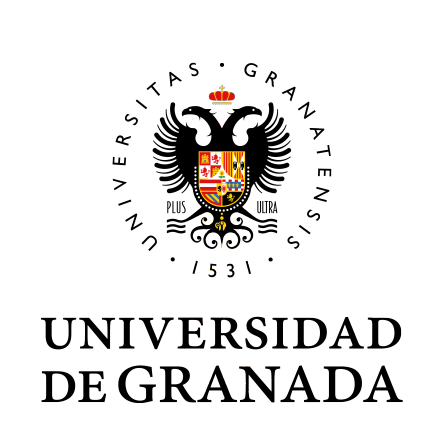
\includegraphics[scale=0.5]{img/ugr.png}\\

\textsc{\Large \asignatura{}\\[0.2cm]}
\textsc{GRADO EN INGENIERÍA INFORMÁTICA}\\[1cm]

\noindent\rule[-1ex]{\textwidth}{1pt}\\[1.5ex]
\textsc{{\Huge \titulo\\[0.5ex]}}
\textsc{{\Large \subtitulo\\}}
\noindent\rule[-1ex]{\textwidth}{2pt}\\[3.5ex]

\end{minipage}

\vspace{0.5cm}

\begin{minipage}{\textwidth}

\centering

\textbf{Autor}\\ {\autor{}}\\[2.5ex]
\textbf{Rama}\\ {Computación y Sistemas Inteligentes}\\[2.5ex]
\vspace{0.3cm}


\includegraphics[scale=0.3]{img/etsiit.jpeg}

\vspace{0.7cm}
\textsc{Escuela Técnica Superior de Ingenierías Informática y de Telecomunicación}\\
\vspace{1cm}
\textsc{Curso 2019-2020}
\end{minipage}
\end{titlepage}

\pagenumbering{arabic}
\tableofcontents
\thispagestyle{empty}				% No usar estilo en la pagina de indice

\newpage

\setlength{\parskip}{1em}


\section*{Ejercicio 1}
\addcontentsline{toc}{section}{Ejercicio 1}

\textbf{Diga en una sola frase cuál cree que es el objetivo principal de la Visión por Computador. Diga también cuál
es la principal propiedad de las imágenes de cara a la creación algoritmos que la procesen.}

El objetivo principal de la Visión por Computador es obtener información significativa de imágenes digitales, posteriormente
analizarla, tratarla y comprender su contenido para tomar decisiones sobre ella de la forma más similar posible a la humana.

Pese a la respresentación en forma matricial de las imágenes que facilita los cálculos a los algoritmos, no podemos centrarnos
únicamente en una posición (píxel) de ésta, ya que los valores alrededor suyo también contienen información relevante sobre él.


\section*{Ejercicio 2}
\addcontentsline{toc}{section}{Ejercicio 2}

\textbf{Expresar las diferencias y semejanzas entre las operaciones de correlación y convolución. Dar una interpretación
de cada una de ellas que en el contexto de uso en visión por computador.}

Ambas son operaciones que transforman localmente una imagen calculado nuevos valores para cada uno de los píxeles. Esto lo hacen
utilizando una máscara 2D de tamaño $NxN$, siendo $N$ un número impar, y aplicándola de la siguiente forma:

Para la correlación:
\begin{equation}
G[i,j]= \sum_{u=-k}^{k} \sum_{v=-k}^{k} H[u,v]F[i+u,j+v]
\end{equation}

Para la convolución:
\begin{equation}
G[i,j]= \sum_{u=-k}^{k} \sum_{v=-k}^{k} H[u,v]F[i-u,j-v]
\end{equation}

Como podemos ver, correlación y convolución son prácticamente iguales, excepto que en la convolución volteamos el filtro antes de
correlacionar. Por ejemplo, convolucionar una imagen 1D con un filtro $(1,3,5)$ sería lo mismo que correlacionarla con el filtro
$(5,3,1)$. En caso de que fuese una convolución 2D voltearíamos tanto horizontal como verticalmente.

Otra cosa que tienen en común es que, como ambos son filtros lineales, ambos cumplen las siguientes propiedades: la \textbf{
superposición}, la cual dice que es lo mismo aplicar una máscara a una composición de imágenes $f_1+f_2$, que aplicarsela a
$f_1$ y a $f_2$ por separado: $h*(f_1 + f_2) = (h*f_1) + (h*f_2)$; y son \textbf{\textit{Shift-Invariant System}}, es decir,
sistemas cuyo valor de entrada no cambian los valores de salida, por lo que no dependen de ellos.

La diferencias más importantes entre ellos es que la convolución es \textbf{conmutativa}, \textbf{distributiva en la adición} y, la
más relevante, \textbf{asociativa}. Es decir, siendo $f$ y $g$ dos filtros distintos, entonces $(f * g)*h = f*(g * h)$. Esto es muy
útil por ejemplo para calcular el filtro \textit{Difference of Gaussian (DoG)}, en el que no tendríamos que convolucionar la imagen
con un filtro Gaussiano y posteriormente con uno derivado, simplemente convolucionaríamos el filtro Gaussiano con el derivado y ya se
lo aplicamos a la imagen.


\section*{Ejercicio 3}
\addcontentsline{toc}{section}{Ejercicio 3}

\textbf{¿Cuál es la diferencia “esencial” entre el filtro de convolución y el de mediana? Justificar la respuesta.}

La principal diferencia entre estos filtros es que el filtro de convolución, como hemos visto antes, es lineal, mientras que el
filtro de mediana no lo es. Para justificar la respuesta veamos un ejemplo: si tenemos los filtros $A=(0,1,2,3,4)$, $B=(5,0,1,4,5)$
y $(A+B)=(5,1,3,7,9)$, el cálculo de sus medianas es:
\begin{equation}
Med(A) = 2 \hspace{10mm} Med(B) = 4
\end{equation}
Y por tanto, como:

\begin{equation}
Med(A)+Med(B)=6 \hspace{5mm} \neq \hspace{5mm} Med(A+B)=5
\end{equation}

podemos justificar que los filtros de mediana no son lineales.

\newpage


\section*{Ejercicio 4}
\addcontentsline{toc}{section}{Ejercicio 4}

\textbf{Identifique el “mecanismo concreto” que usa un filtro de máscara para transformar una imagen.}

El mecanismo que utilizan todos los filtros de máscara para transformar una imagen es que lo hace utilizando \textbf{información local},
es decir, que el valor de cada píxel se calcula teniendo en cuenta los píxeles cercanos a él (los que están dentro de la máscara).

Podremos encontrar varios tipos de filtros, ya sean lineales o no lineales como hemos visto antes, pero ninguno realizará cálculos
en la imagen sin tener en cuenta sus píxeles asociados en la máscara.

\section*{Ejercicio 5}
\addcontentsline{toc}{section}{Ejercicio 5}

\textbf{¿De qué depende que una máscara de convolución pueda ser implementada por convoluciones 1D? Justificar la respuesta.}

Depende de que la máscara de convolución solo se pueda descomponer como producto de dos matrices de dimensión 1. Por ejemplo,
la siguiente máscara Gaussiana se puede descomponer en:

\begin{equation}
\begin{bmatrix}
1 & 2 & 1\\ 
2 & 4 & 2\\ 
1 & 2 & 1
\end{bmatrix}
=
\begin{bmatrix}
1\\
2\\
1
\end{bmatrix}
\begin{bmatrix}
1 & 2 & 1
\end{bmatrix}
\end{equation}


Para comprobar si esto es posible, podemos realizar la \textbf{descomposición en valores singulares} de la matriz. Si esta
descomposición nos da un valor distinto de 0, la máscara será separable en dos matrices 1D, y por tanto, la podremos represetar
como:
\begin{equation}
\sum_{r}^{i=0}\sigma_i u_i v_i^T
\end{equation}
siendo $\sigma_i$ los valores de la matriz diagonal, y $u_i$ y $v_i$ los valores de las respectivas matrices 1D resultantes.

Otra forma que tenemos de comprobarlo es que, si nos fijamos en este tipo de máscaras, el \textbf{rango} de la matriz siempre va
a ser igual a 1.


\section*{Ejercicio 6}
\addcontentsline{toc}{section}{Ejercicio 6}

\textbf{Identificar las diferencias y consecuencias desde el punto de vista teórico y de la implementación entre:}
\begin{enumerate}[label=(\alph*)]
	\item \textbf{Primero alisar la imagen y después calcular las derivadas sobre la imagen alisada}
	\item \textbf{Primero calcular las imágenes derivadas y después alisar dichas imágenes.}
\end{enumerate}
\textbf{Justificar los argumentos.}

Desde un punto de vista teórico dependerá del tipo de filtro que usemos, pero lo lógico sería elegir un filtro de convolución.
Como hemos visto en el ejercicio 2, este filtro tiene cumple la propiedad \textbf{asociativa}, por lo que tanto la opción $a$ como
la $b$ darían el mismo resultado.

\begin{equation}
(f*g)*h=f*(g*h)
\end{equation}

En cuanto a la implementación, es más conveniente \textbf{alisar primero la imagen y posteriormente calcular las derivadas} sobre
la imagen alisada. Si lo hacemos de esta forma, tendremos que hacer solo una convolución y dos derivadas después. De la otra forma,
haremos dos derivadas al principio y posteriormente dos alisamientos, uno para la X y otro para la Y.


\section*{Ejercicio 7}
\addcontentsline{toc}{section}{Ejercicio 7}

\textbf{}


\section*{Ejercicio 8}
\addcontentsline{toc}{section}{Ejercicio 8}


\section*{Ejercicio 9}
\addcontentsline{toc}{section}{Ejercicio 9}


\section*{Ejercicio 10}
\addcontentsline{toc}{section}{Ejercicio 10}


\section*{Ejercicio 11}
\addcontentsline{toc}{section}{Ejercicio 11}

\textbf{¿Bajo qué condiciones podemos garantizar una perfecta reconstrucción de una imagen a partir de su pirámide Laplaciana? Dar
argumentos y discutir las opciones que considere necesario.}

Únicamente con la pirámide Laplaciana no podríamos reconstruir la imagen original, también necesitaríamos la última submuestra de
la imagen obtenida al hacer la pirámide Gaussiana.

Si disponemos de ella, se podría reconstruir con el siguiente algoritmo, el cual consiste en sumar al último nivel de la Laplaciana
esta última submuestra de la Gaussiana ampliada con una función F:
\begin{equation}
G_k=L_k+F(G_{k+1})
\end{equation}

Cuando terminemos (llegemos a $G_1$) será cuando tengamos la imagen original completamente reconstruida.

\section*{Ejercicio 12}
\addcontentsline{toc}{section}{Ejercicio 12}

\textbf{¿Cuáles son las contribuciones más relevantes del algoritmo de Canny al cálculo de los contornos sobre una imagen? ¿Existe
alguna conexión entre las máscaras de Sobel y el algoritmo de Canny? Justificar la respuesta}

Las contribuciones que tiene este algoritmo frente a otros es que este utiliza las siguientes técnicas:
\begin{enumerate}
	\item \textbf{Non-maximum supression.} Esta técnica recorre todos los píxeles de cada imagen y, para cada uno de ellos, comprueba
	que sus píxeles fronterizos no tienen un valor más alto que el central. En caso de que exista, lo pondrá este a cero.
			\begin{equation*}
				\begin{bmatrix}
				3& 2& 3\\ 
				6& 4& 1\\ 
				1& 3& 3
				\end{bmatrix}
				\underset{(x,y)>=(0,0)}{\rightarrow}
				\begin{bmatrix}
				3& 2& 3\\ 
				6& 0& 1\\ 
				1& 3& 3
				\end{bmatrix}
				\hspace{10mm}
				\begin{bmatrix}
				3& 2& 3\\ 
				1& 4& 1\\ 
				1& 3& 3
				\end{bmatrix}
				\underset{(x,y)<(0,0)}{\rightarrow}
				\begin{bmatrix}
				0& 0& 0\\ 
				0& 4& 0\\ 
				0& 0& 0
				\end{bmatrix}
			\end{equation*}
	Para tener más claro cómo funciona este algoritmo, vamos a ejemplificarlo con una matriz ejemplo que represente los píxeles de una imagen.


	\item dskjfjegnjdgbffjb
\end{enumerate}


\section*{Ejercicio 13}
\addcontentsline{toc}{section}{Ejercicio 13}


\section*{Ejercicio 14}
\addcontentsline{toc}{section}{Ejercicio 14}


\section*{Ejercicio 15}
\addcontentsline{toc}{section}{Ejercicio 15}


\end{document}